
\subsection{Programtest}
Først testes metoden, der får input fra brugeren:

\begin{lstlisting}
Type size for canvas: fisk
This is not an integer, using default of: 512
Type size of walk: -5
This is not a positive integer, using default of: 50
Debug mode? "y" for yes: n
Entering regular mode
Type "exit" to stop, anything else to draw a new walk: exit
Quitting
Program terminated
\end{lstlisting}
Det ses at både ord og negative tal forkastes. Skærm-outputtet til dette kan ses i figur~\ref{fig:walkM}

\begin{figure}[h!]
	\centering
	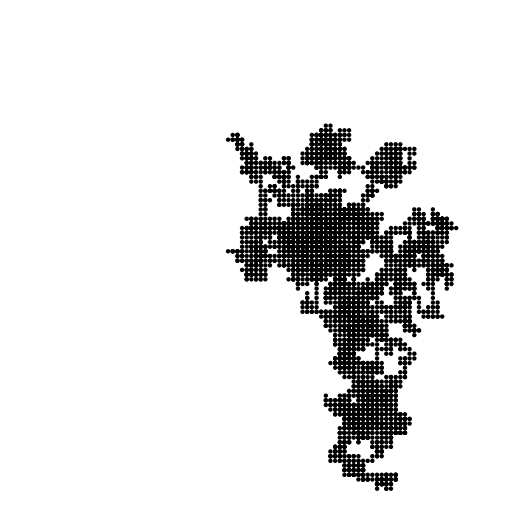
\includegraphics[width=0.5\textwidth]{walkM}
		\caption{Randomwalk med gitter på 101x101 og en opløsning på 512x512px}\label{fig:walkM}
\end{figure}

Dernæst testes debug print af position:
\begin{lstlisting}
Type size for canvas: 512
Type size of walk: 10
Debug mode? "y" for yes: y
Entering debug mode
Position: (0, 1)
Position: (-1, 1)
Position: (-1, 2)
... og mange flere ...
Position: (1, 10)
Position: (0, 10)
Position: (1, 10)
Type "exit" to stop, anything else to draw a new walk: exit
Quitting
Program terminated
\end{lstlisting}
Det ses at ``turisten''/''støvpartiklen''s position printes til konsollen. Skærm-outputtet til dette kan ses i figur~\ref{fig:walkS}

\begin{figure}[h!]
	\centering
	
\includegraphics[width=0.5\textwidth]{walkS}
		\caption{Randomwalk med gitter på 21x21 og en opløsning på 512x512px}\label{fig:walkS}
\end{figure}

Til slut testes et gigantisk randomwalk, billed størrelsen er 4500x4500px og der gåes på et gitter på 2001x2001. Resultatet er i figur~\ref{fig:walkH}

\begin{figure}[h!]
	\centering
	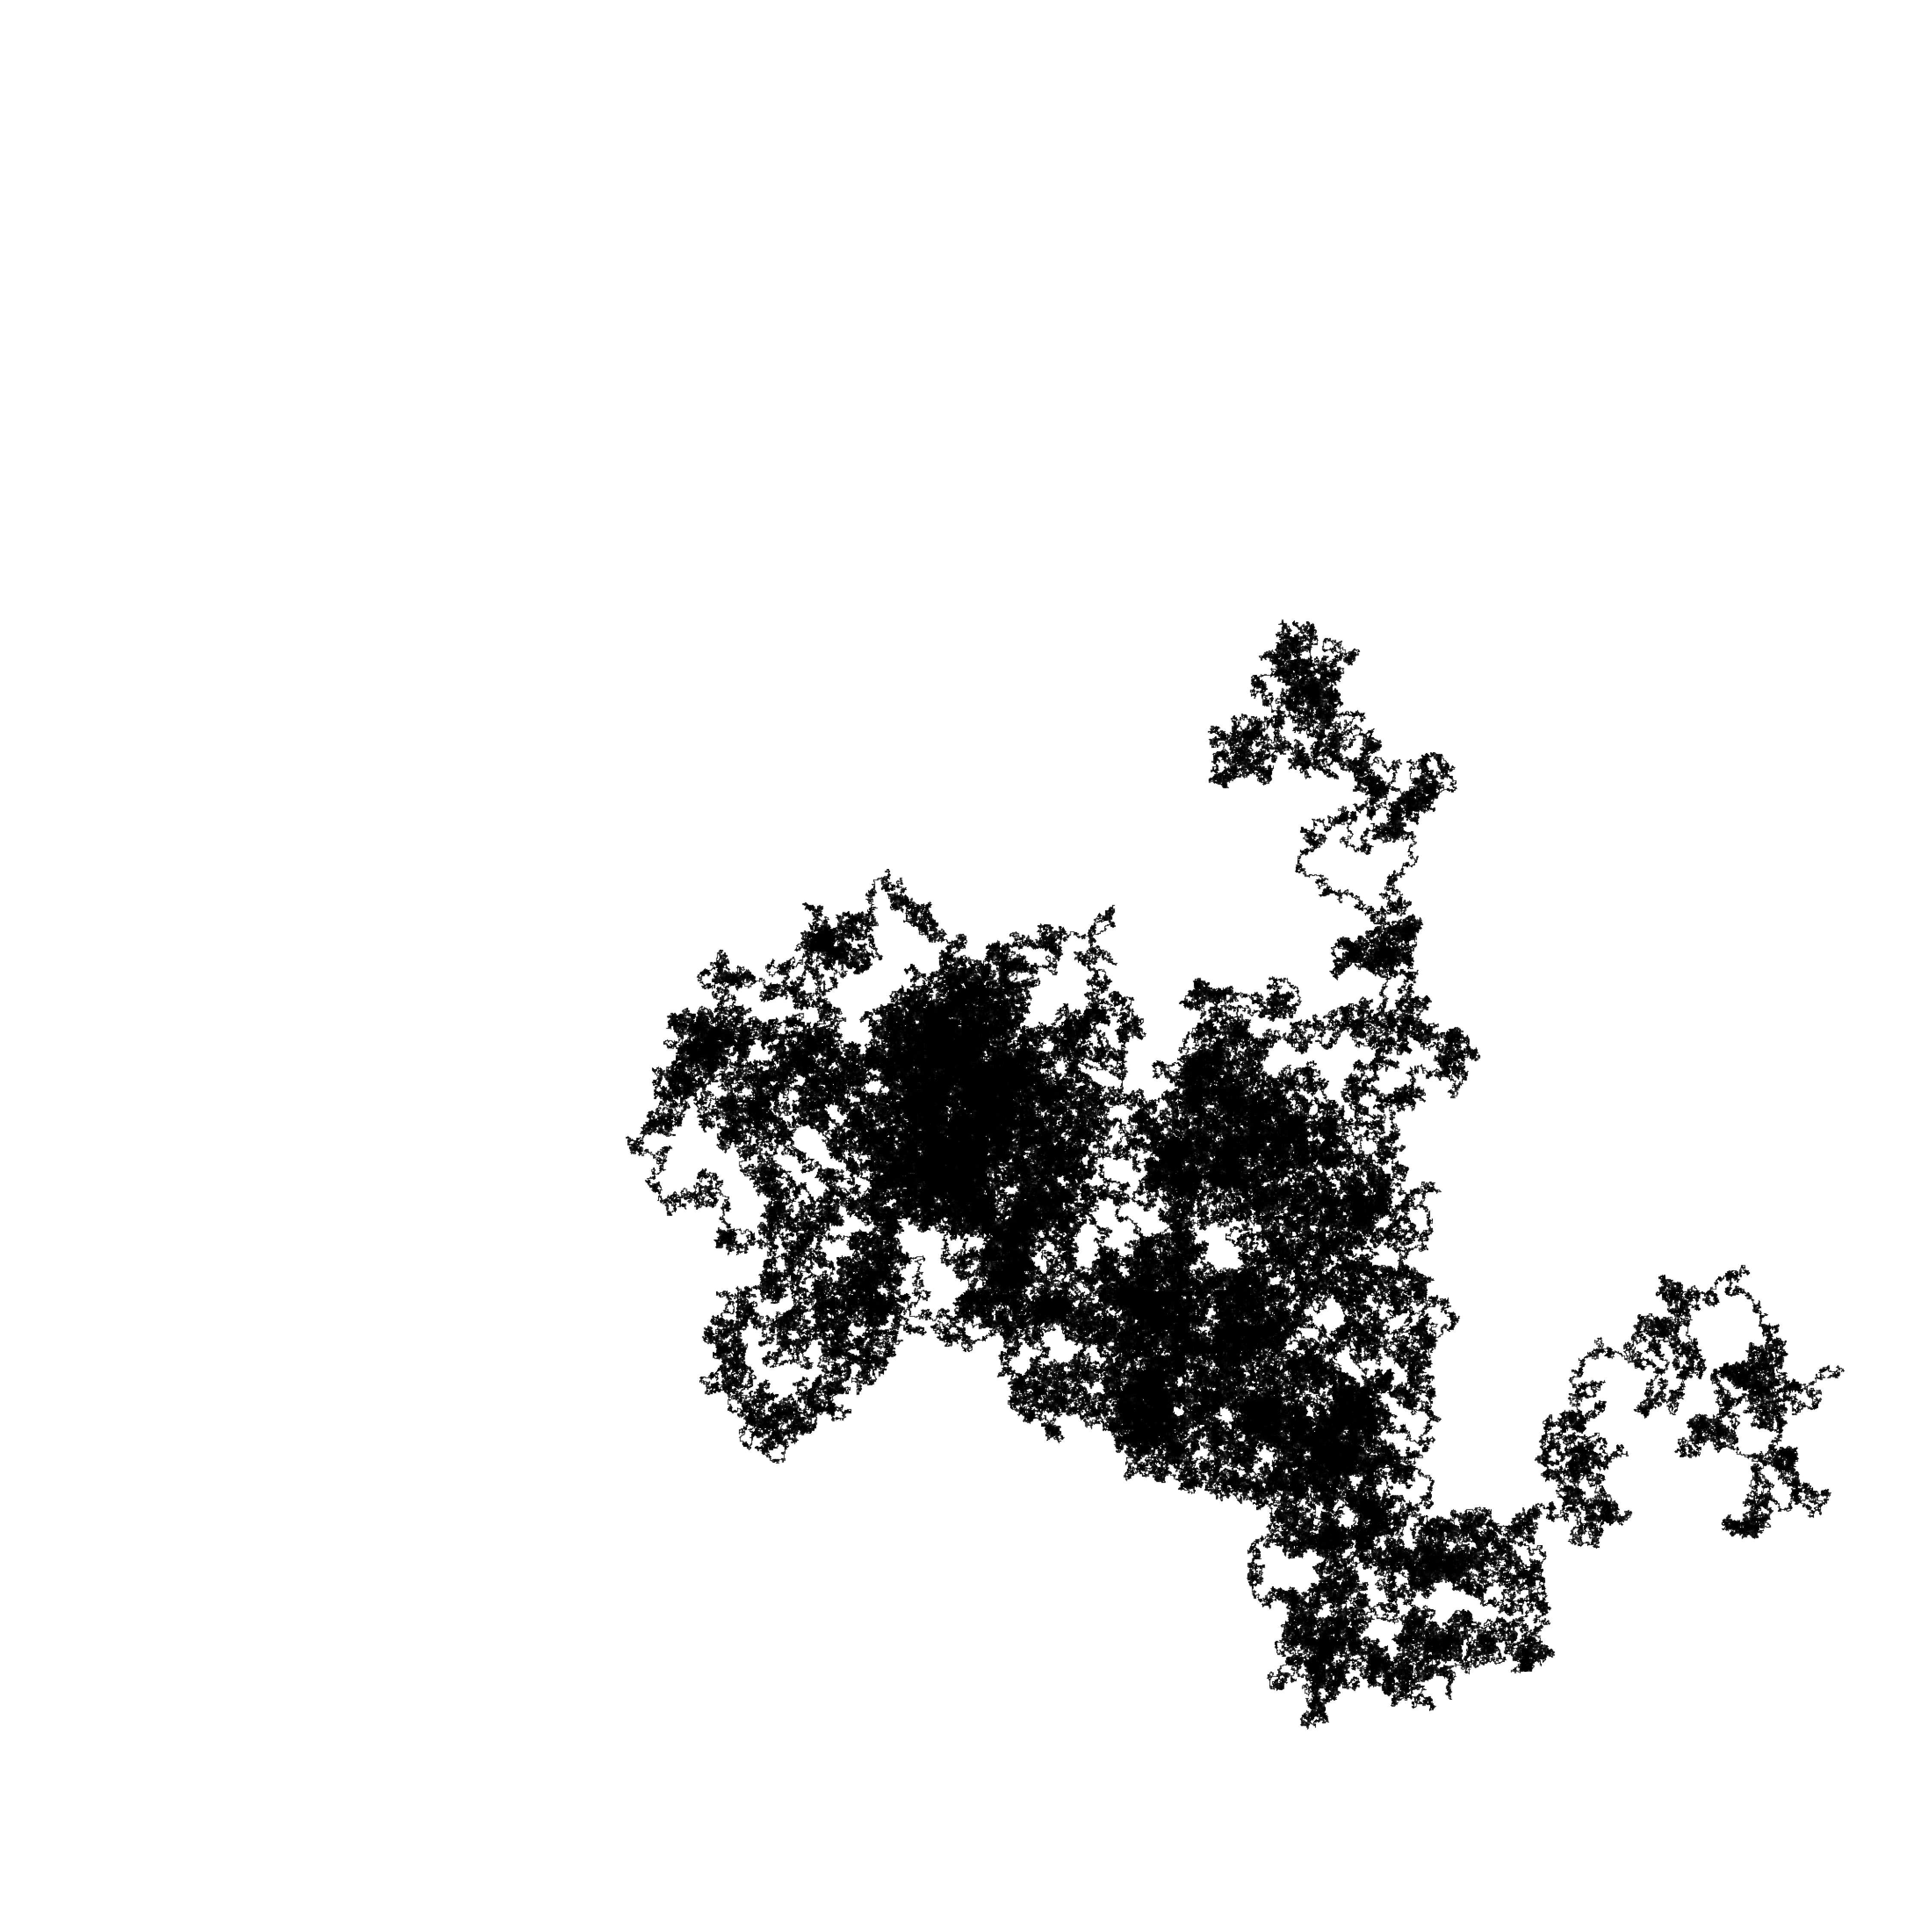
\includegraphics[width=0.9\textwidth]{walkH}
		\caption{Randomwalk med gitter på 2001x2001 og en opløsning på 4500x4500px}\label{fig:walkH}
\end{figure}